\documentclass[11pt,a4paper]{article}
% Document formatting
\usepackage[margin=2.5cm]{geometry}
\usepackage{amsmath}
\usepackage{amssymb}
\usepackage{graphicx}
\usepackage{booktabs}
\usepackage{float}
\usepackage[hidelinks]{hyperref}\usepackage{setspace}
\onehalfspacing
% Figures are stored outside the report folder
\graphicspath{{results/}}
\title{\textbf{Double Descent in Linear Models}\\[0.5cm]
\large Statistical Methods for Machine Learning}
\author{Sanim Mazhit\\ Academic Year 2025/2026}
\date{\today}
\begin{document}
\maketitle

\begin{abstract}
This project investigates the double descent phenomenon in
linear regression. We study how training and test errors
change as the number of features increases, with particular
attention to the interpolation threshold.
We implement least squares and ridge regression using
NumPy and evaluate them on synthetic regression data and
the California Housing dataset. We also examine the
effects of regularization, label noise, and random variation
across experimental runs.
\end{abstract}

\tableofcontents
\newpage
% Report sections will be added below

\section{Introduction}
In classical machine learning, increasing model complexity
can improve performance at first, but may eventually lead
to overfitting. This is commonly described using the
bias-variance trade-off.
However, recent research has shown that some models behave
differently when their complexity becomes sufficiently
large. Instead of following a single U-shaped test-error
curve, they can exhibit a phenomenon known as
\textit{double descent} \cite{belkin2019}.
In double descent, test error initially decreases,
then increases sharply near the interpolation threshold,
and may decrease again when the model becomes
overparameterized.
The objective of this project is to investigate this
behavior in linear regression through numerical experiments.
We focus on three research questions:
\begin{enumerate}
    \item How does test error change when the number of
    features increases relative to the number of
    training observations?
    \item How does ridge regularization affect the
    interpolation peak and generalization error?
    \item How do label noise and data characteristics
    influence the double descent phenomenon?
\end{enumerate}

We study these questions using synthetic regression data
and the California Housing dataset.

\section{Theoretical Background}

\subsection{Linear Regression}
Consider a regression dataset with $n$ observations
and $d$ features.
The feature matrix is
$X \in \mathbb{R}^{n \times d}$,
and the target vector is
$y \in \mathbb{R}^{n}$.
A linear model predicts the targets using
\begin{equation}
    \hat{y} = Xw,
\end{equation}
where $w \in \mathbb{R}^{d}$ is the vector of
model parameters.
The goal is to find parameters that minimize the
difference between predicted and observed values.

\subsection{Least Squares Regression}
Ordinary least squares minimizes the squared
prediction error:
\begin{equation}
    \hat{w}_{LS}
    =
    \arg\min_w
    \|Xw-y\|_2^2.
\end{equation}
When the system is overparameterized, there may be
multiple solutions that fit the training data exactly.
We use the Moore-Penrose pseudoinverse to obtain
a minimum-norm least-squares solution:
\begin{equation}
    \hat{w}_{LS} = X^{+}y.
\end{equation}
This solution is computed using NumPy's pseudoinverse
operation in our implementation.

\subsection{Ridge Regression}
Ridge regression introduces an $L_2$ penalty on
the model parameters:
\begin{equation}
    \hat{w}_{Ridge}
    =
    \arg\min_w
    \left(
    \|Xw-y\|_2^2
    +
    \alpha \|w\|_2^2
    \right),
\end{equation}
where $\alpha > 0$ controls the strength of
regularization.
The corresponding solution is
\begin{equation}
    \hat{w}_{Ridge}
    =
    (X^\top X + \alpha I)^{-1}X^\top y.
\end{equation}
In our implementation, we solve the corresponding
linear system numerically instead of explicitly
computing the matrix inverse.
Regularization discourages very large coefficients
and can improve generalization, particularly when
the least-squares solution is unstable.

\subsection{The Double Descent Phenomenon}
The interpolation threshold is reached when the
model has sufficient capacity to fit the training
observations exactly.
For the regression designs considered in this project,
the threshold occurs near $d=n$, where $d$ is the
number of features and $n$ is the number of
training samples.
Near this threshold, the feature matrix can become
poorly conditioned. Consequently, the least-squares
solution may have a large coefficient norm and
produce a sharp increase in test error.
When the number of features increases further,
the minimum-norm solution can become more stable,
and test error may decrease again.
This second decrease is the defining feature of
the double descent phenomenon.

\subsection{Evaluation Metric}
We evaluate prediction performance using mean
squared error (MSE):
\begin{equation}
    \mathrm{MSE}
    =
    \frac{1}{m}
    \sum_{i=1}^{m}
    (y_i-\hat{y}_i)^2,
\end{equation}
where $m$ is the number of observations
in the evaluated dataset.
We report training MSE to measure how well
the model fits the training observations,
and test MSE to evaluate generalization
to unseen observations.

\section{Experimental Methodology}
This section describes the implementation, datasets,
experimental settings, and evaluation procedure.
All experiments were implemented in Python using NumPy
for numerical computations. Scikit-learn was used for
dataset loading, preprocessing, and data splitting.
The regression algorithms themselves were implemented
from scratch.

\subsection{Regression Implementations}
Least squares regression was implemented using the
Moore-Penrose pseudoinverse:
\begin{equation}
    \hat{w}_{LS} = X^{+}y.
\end{equation}
Ridge regression was implemented by solving
\begin{equation}
    (X^\top X+\alpha I)\hat{w}_{Ridge}=X^\top y.
\end{equation}
Both implementations were checked against reference
numerical implementations in underparameterized
and overparameterized settings.

\subsection{Synthetic Data Generation}
The synthetic experiments use randomly generated
Gaussian features. The training and test feature
matrices are sampled independently from a
standard normal distribution.
Targets follow the linear model
\begin{equation}
    y = Xw^*+\varepsilon,
\end{equation}
where $w^*$ is the true coefficient vector and
$\varepsilon$ represents Gaussian label noise.
We considered two signal structures.
\textbf{Sparse signal:}
Only the first 20 coefficients of $w^*$ are
nonzero. The remaining features contain no
additional signal.
\textbf{Dense signal:}
All coefficients are randomly generated and
the coefficient vector is normalized to have
unit Euclidean norm.
For the main synthetic double descent experiments,
we used 80 training observations and 500 test
observations.
The feature dimension was varied while keeping
the training sample size fixed.
In the dense-signal experiment, the maximum
feature dimension was 500, and the default
noise standard deviation was 0.5.

\subsection{Repeated Experiments and Noise}
To investigate the sensitivity of the results
to randomness, the dense-signal experiment
was repeated using 10 random seeds.
We summarized the resulting test errors using
the mean and median across runs.
We also examined the effect of label noise
using standard deviations of 0.1, 0.5, and 1.0.
For this experiment, we compared feature
dimensions 40, 80, 120, and 300 while keeping
the random seed fixed.
This noise comparison is exploratory and does
not measure variability across different seeds.

\subsection{California Housing Dataset}
For the real-world experiment, we used the
California Housing regression dataset,
which contains eight original input features.
We constructed a subset containing 100 training
observations, 30 validation observations, and
500 test observations.
The remaining observations were not used.
Feature standardization was performed using
the training set statistics. The resulting
transformation was then applied to validation
and test observations.
This prevents information from the validation
or test distributions from influencing the
scaling parameters.

\subsection{Random Fourier Features}
Because the original California Housing dataset
has only eight input features, we used Random
Fourier Features to increase model complexity.
The transformed features were computed as
\begin{equation}
    Z = \cos(XW+b),
\end{equation}
where $W$ is a randomly generated projection
matrix and $b$ contains random phase offsets.
We generated up to 300 transformed features
and varied the number of features included
in each regression model.
The training sample size remained fixed at 100,
so the interpolation threshold was expected
near $d=100$.
The same random feature transformation was
used for the training, validation, and
test observations.

\subsection{Ridge Hyperparameter Selection}
Ridge regularization was evaluated using
a fixed parameter $\alpha=1$ and through
validation-based hyperparameter selection.
For the California Housing experiments,
the candidate values were
\begin{equation}
    \alpha \in
    \{0.01,\ 0.1,\ 1,\ 10,\ 100\}.
\end{equation}
For each feature dimension, the model was
trained on the training set and evaluated
on the validation set.
The value minimizing validation MSE was
selected. Test MSE was then calculated
using the selected parameter.
The test set was not used directly
for selecting the regularization parameter.

\subsection{Evaluation Procedure}
We measured training and test mean squared
error as functions of feature dimension.
For least squares, we examined the behavior
of test error near the interpolation threshold
and in the overparameterized regime.
We also compared least squares with ridge
regression to investigate whether regularization
reduced the interpolation peak.
Random seeds were fixed where appropriate
to make individual experimental runs reproducible.

\section{Synthetic Experimental Results}
We first investigated double descent using synthetic
Gaussian regression data. The experiments considered
both sparse and dense signal structures, with the
number of training observations fixed at $n=80$.

\subsection{Double Descent with a Dense Signal}
Figure~\ref{fig:synthetic_dd} shows the test error of
least squares regression as the number of features
increases.

\begin{figure}[htbp]
    \centering
    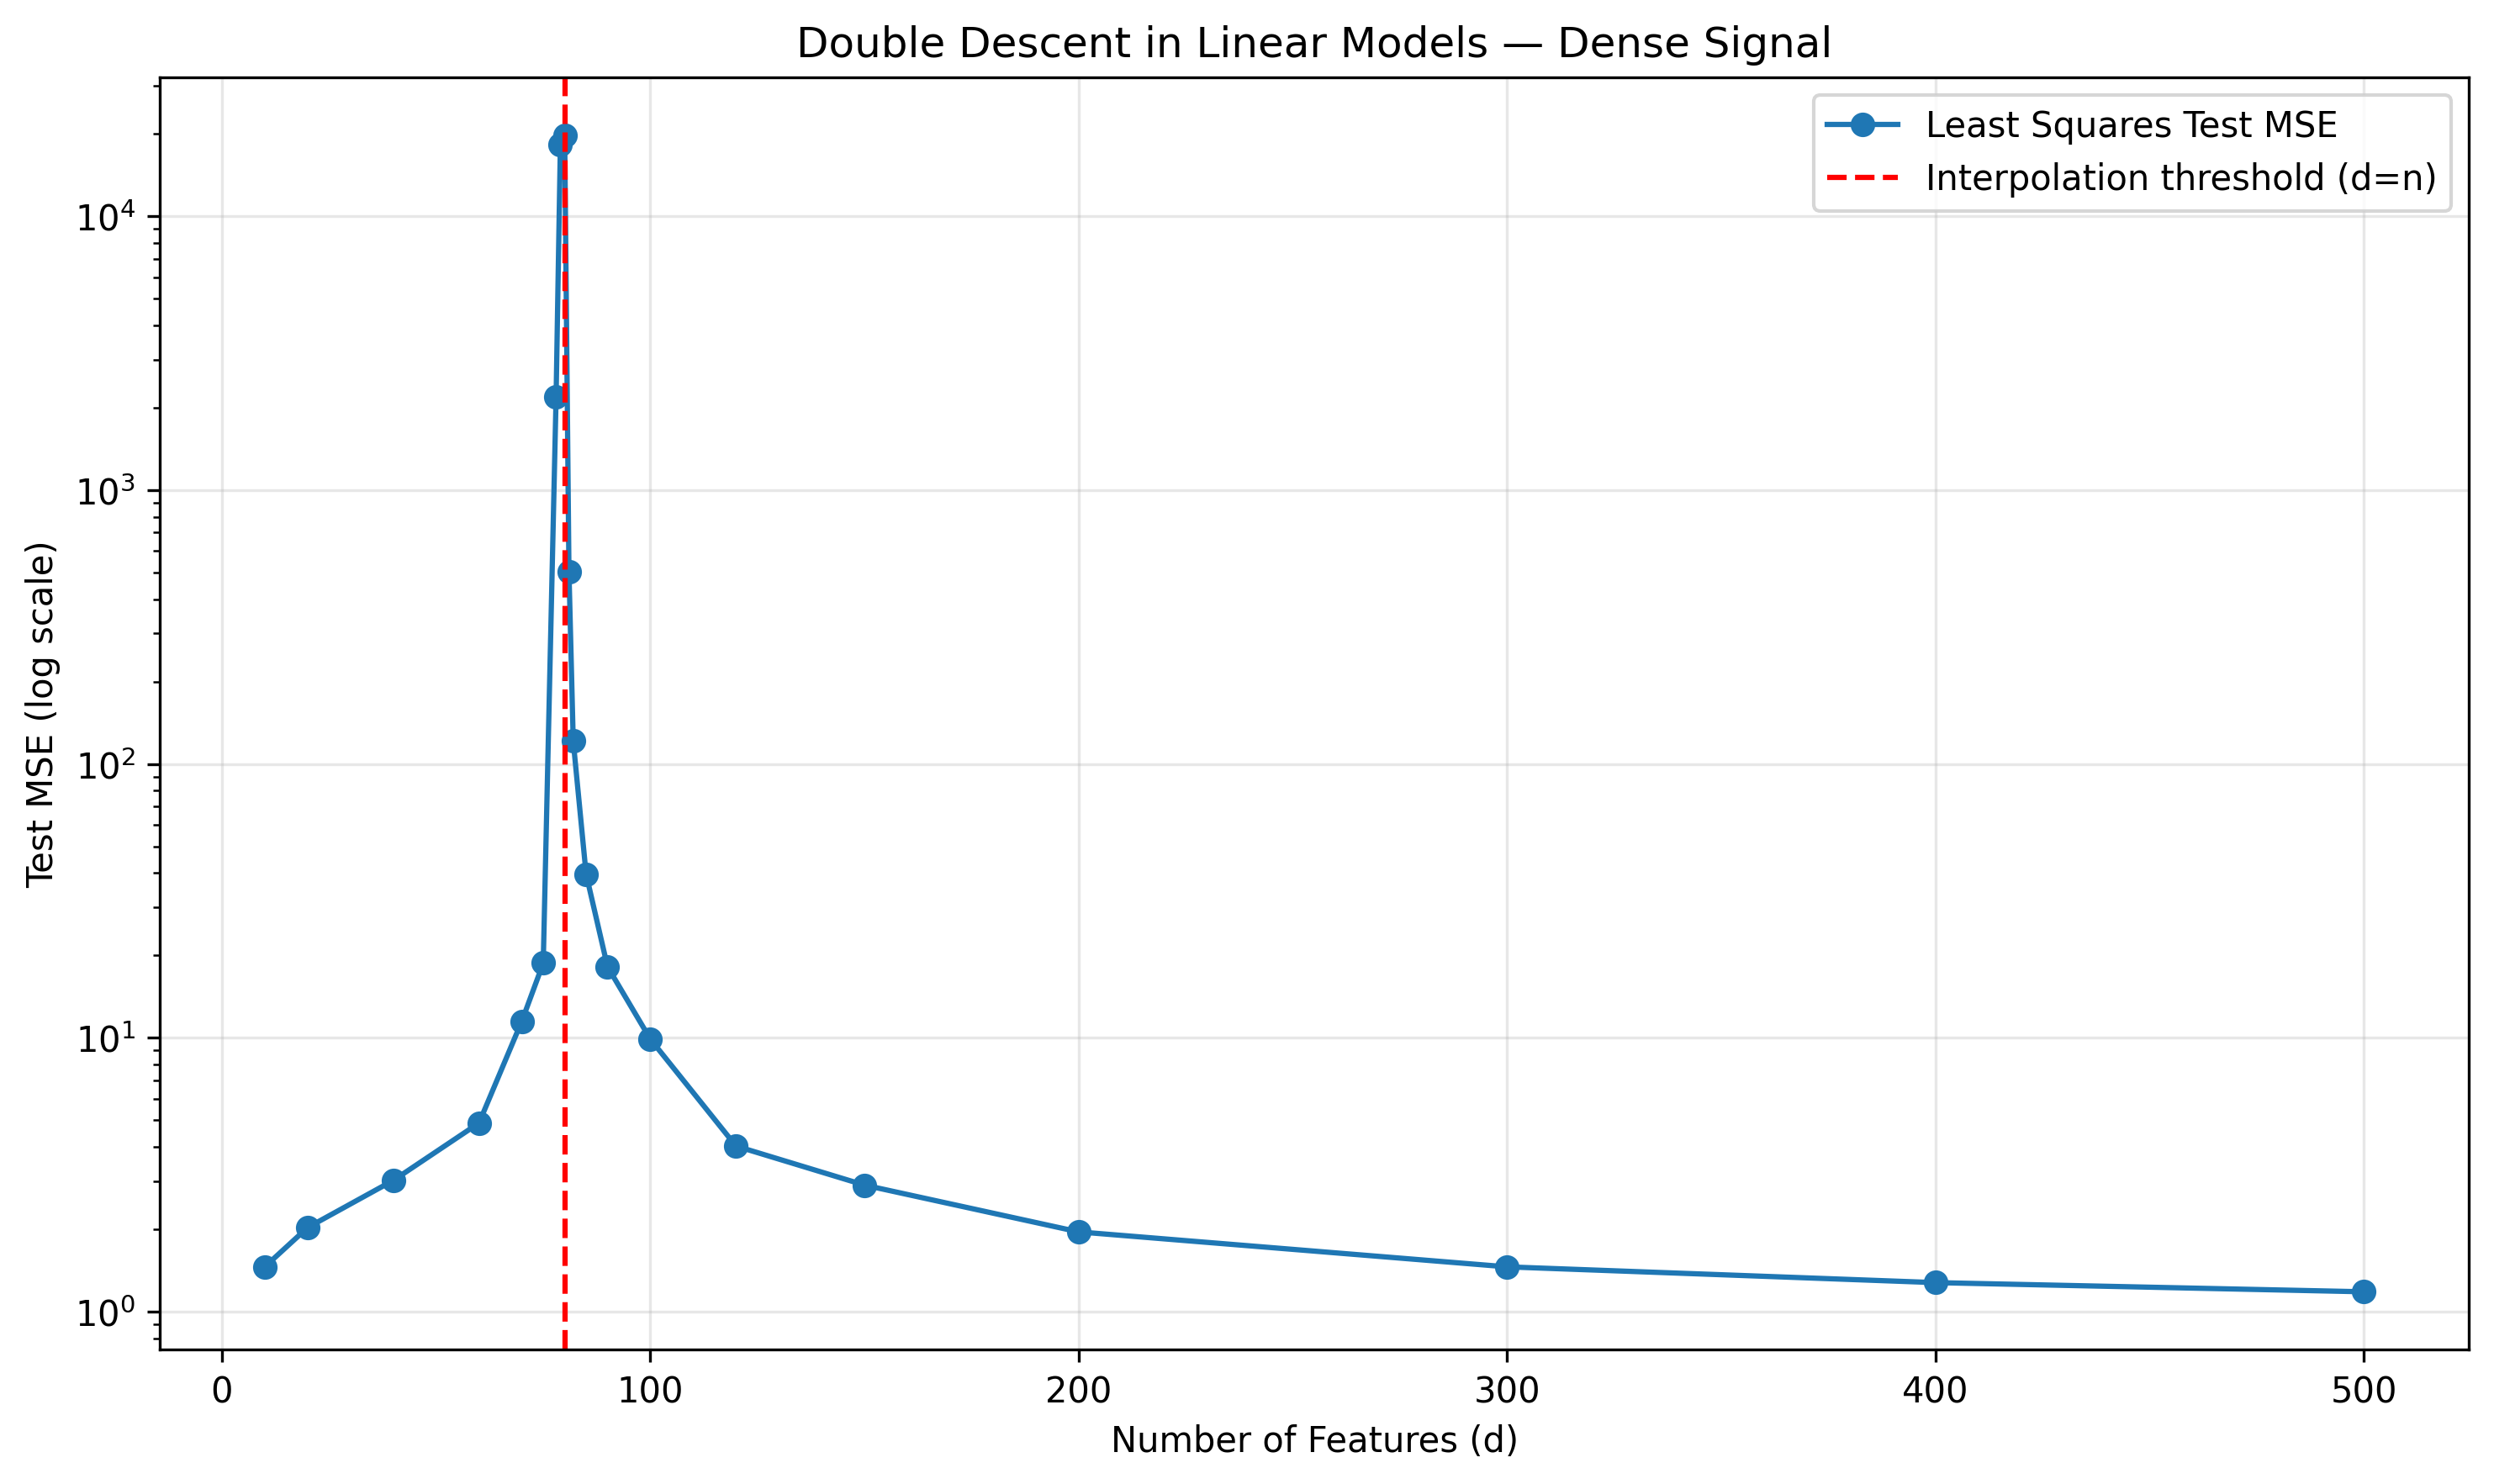
\includegraphics[width=0.85\textwidth]
    {synthetic_double_descent.png}
    \caption{Double descent in the dense-signal
    synthetic experiment. The interpolation threshold
    occurs at $d=80$. The vertical axis uses a
    logarithmic scale.}
    \label{fig:synthetic_dd}
\end{figure}

The results show a pronounced interpolation peak.
With 80 training observations and 80 features,
least squares produces a test MSE of approximately
$19{,}795.6$.
This large error is consistent with numerical
instability near the interpolation threshold,
where the design matrix can become poorly
conditioned.
When the number of features increases beyond
the threshold, the test error decreases
substantially.
At $d=500$, the test MSE is approximately $1.18$.
These results provide a clear example of the
double descent phenomenon.

\subsection{Comparison with Ridge Regression}
We compared the minimum-norm least squares solution
with ridge regression using a fixed regularization
parameter $\alpha=1$.

\begin{figure}[htbp]
    \centering
    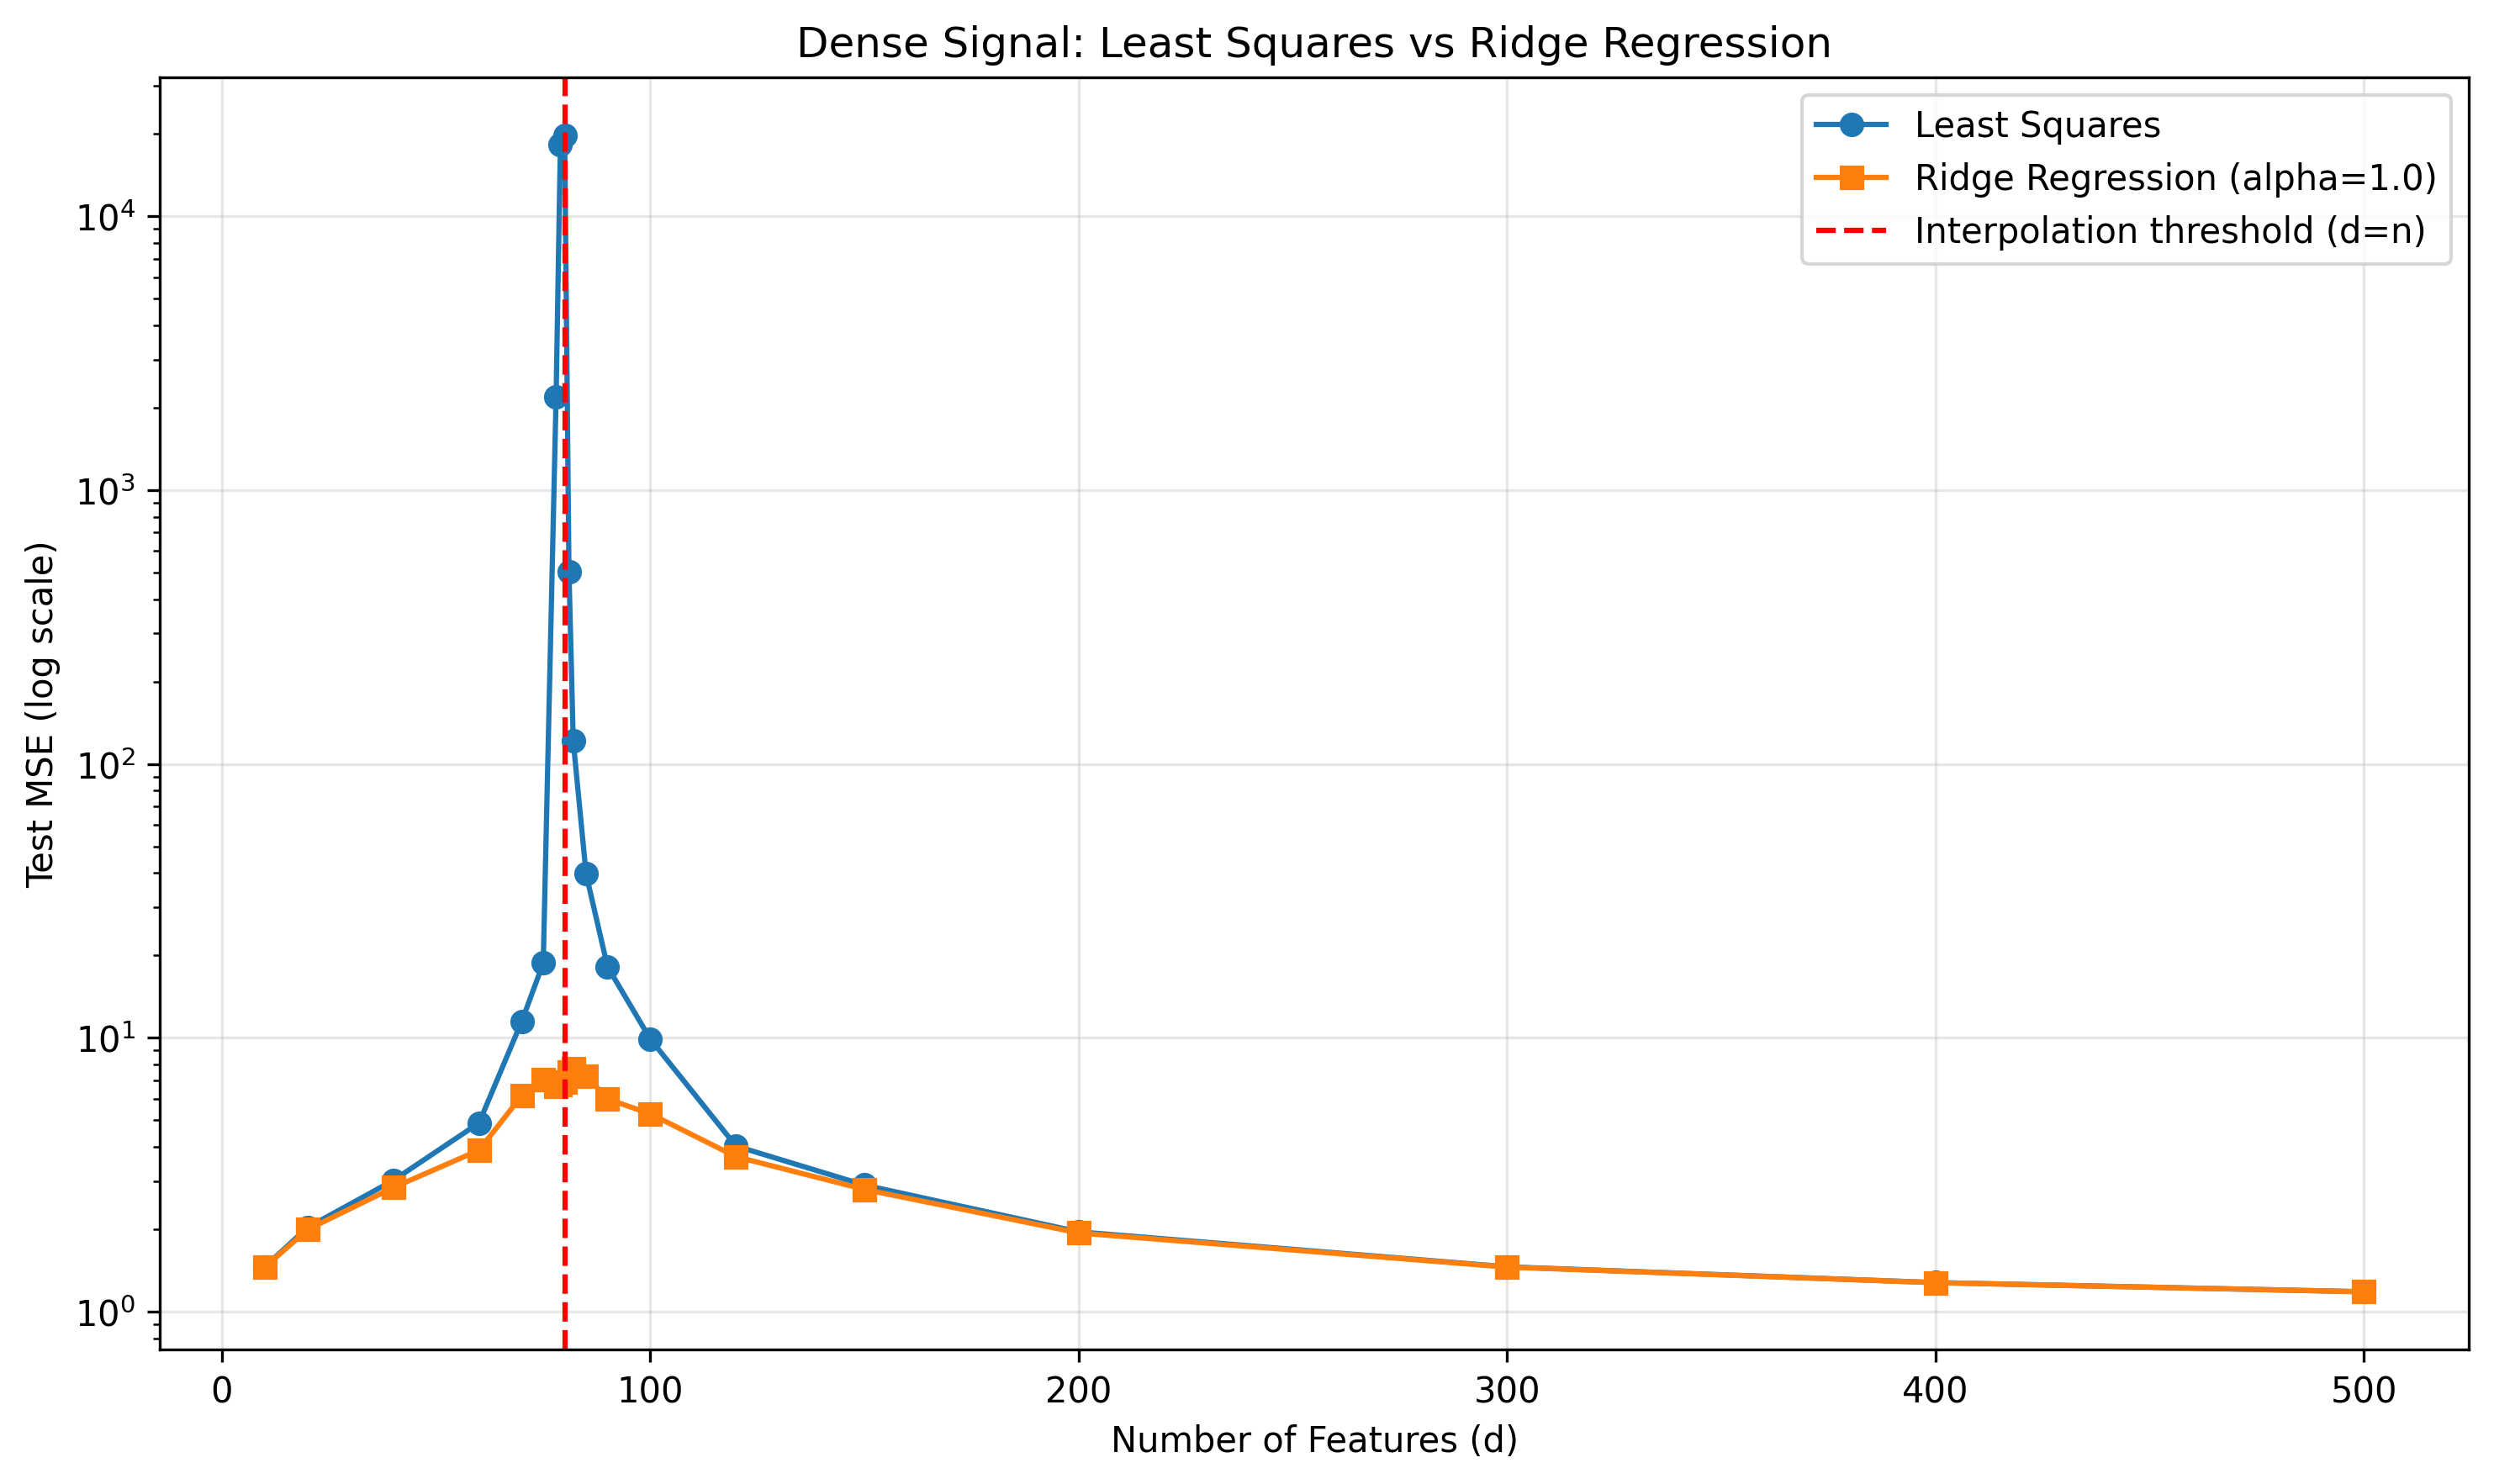
\includegraphics[width=0.85\textwidth]
    {synthetic_ridge_comparison.png}
    \caption{Comparison of least squares and
    ridge regression on dense-signal synthetic data.}
    \label{fig:synthetic_ridge}
\end{figure}

At the interpolation threshold, ridge regression
reduces test MSE from approximately $19{,}795.6$
to $6.90$.
This demonstrates how regularization can reduce
the instability of least squares near
interpolation.
At larger feature dimensions, the difference
between the two methods becomes much smaller
in this experiment.

\subsection{Repeated Experiments}
To investigate whether the observed behavior
depends on a particular random sample, we
repeated the dense-signal experiment using
10 different random seeds.

\begin{figure}[htbp]
    \centering
    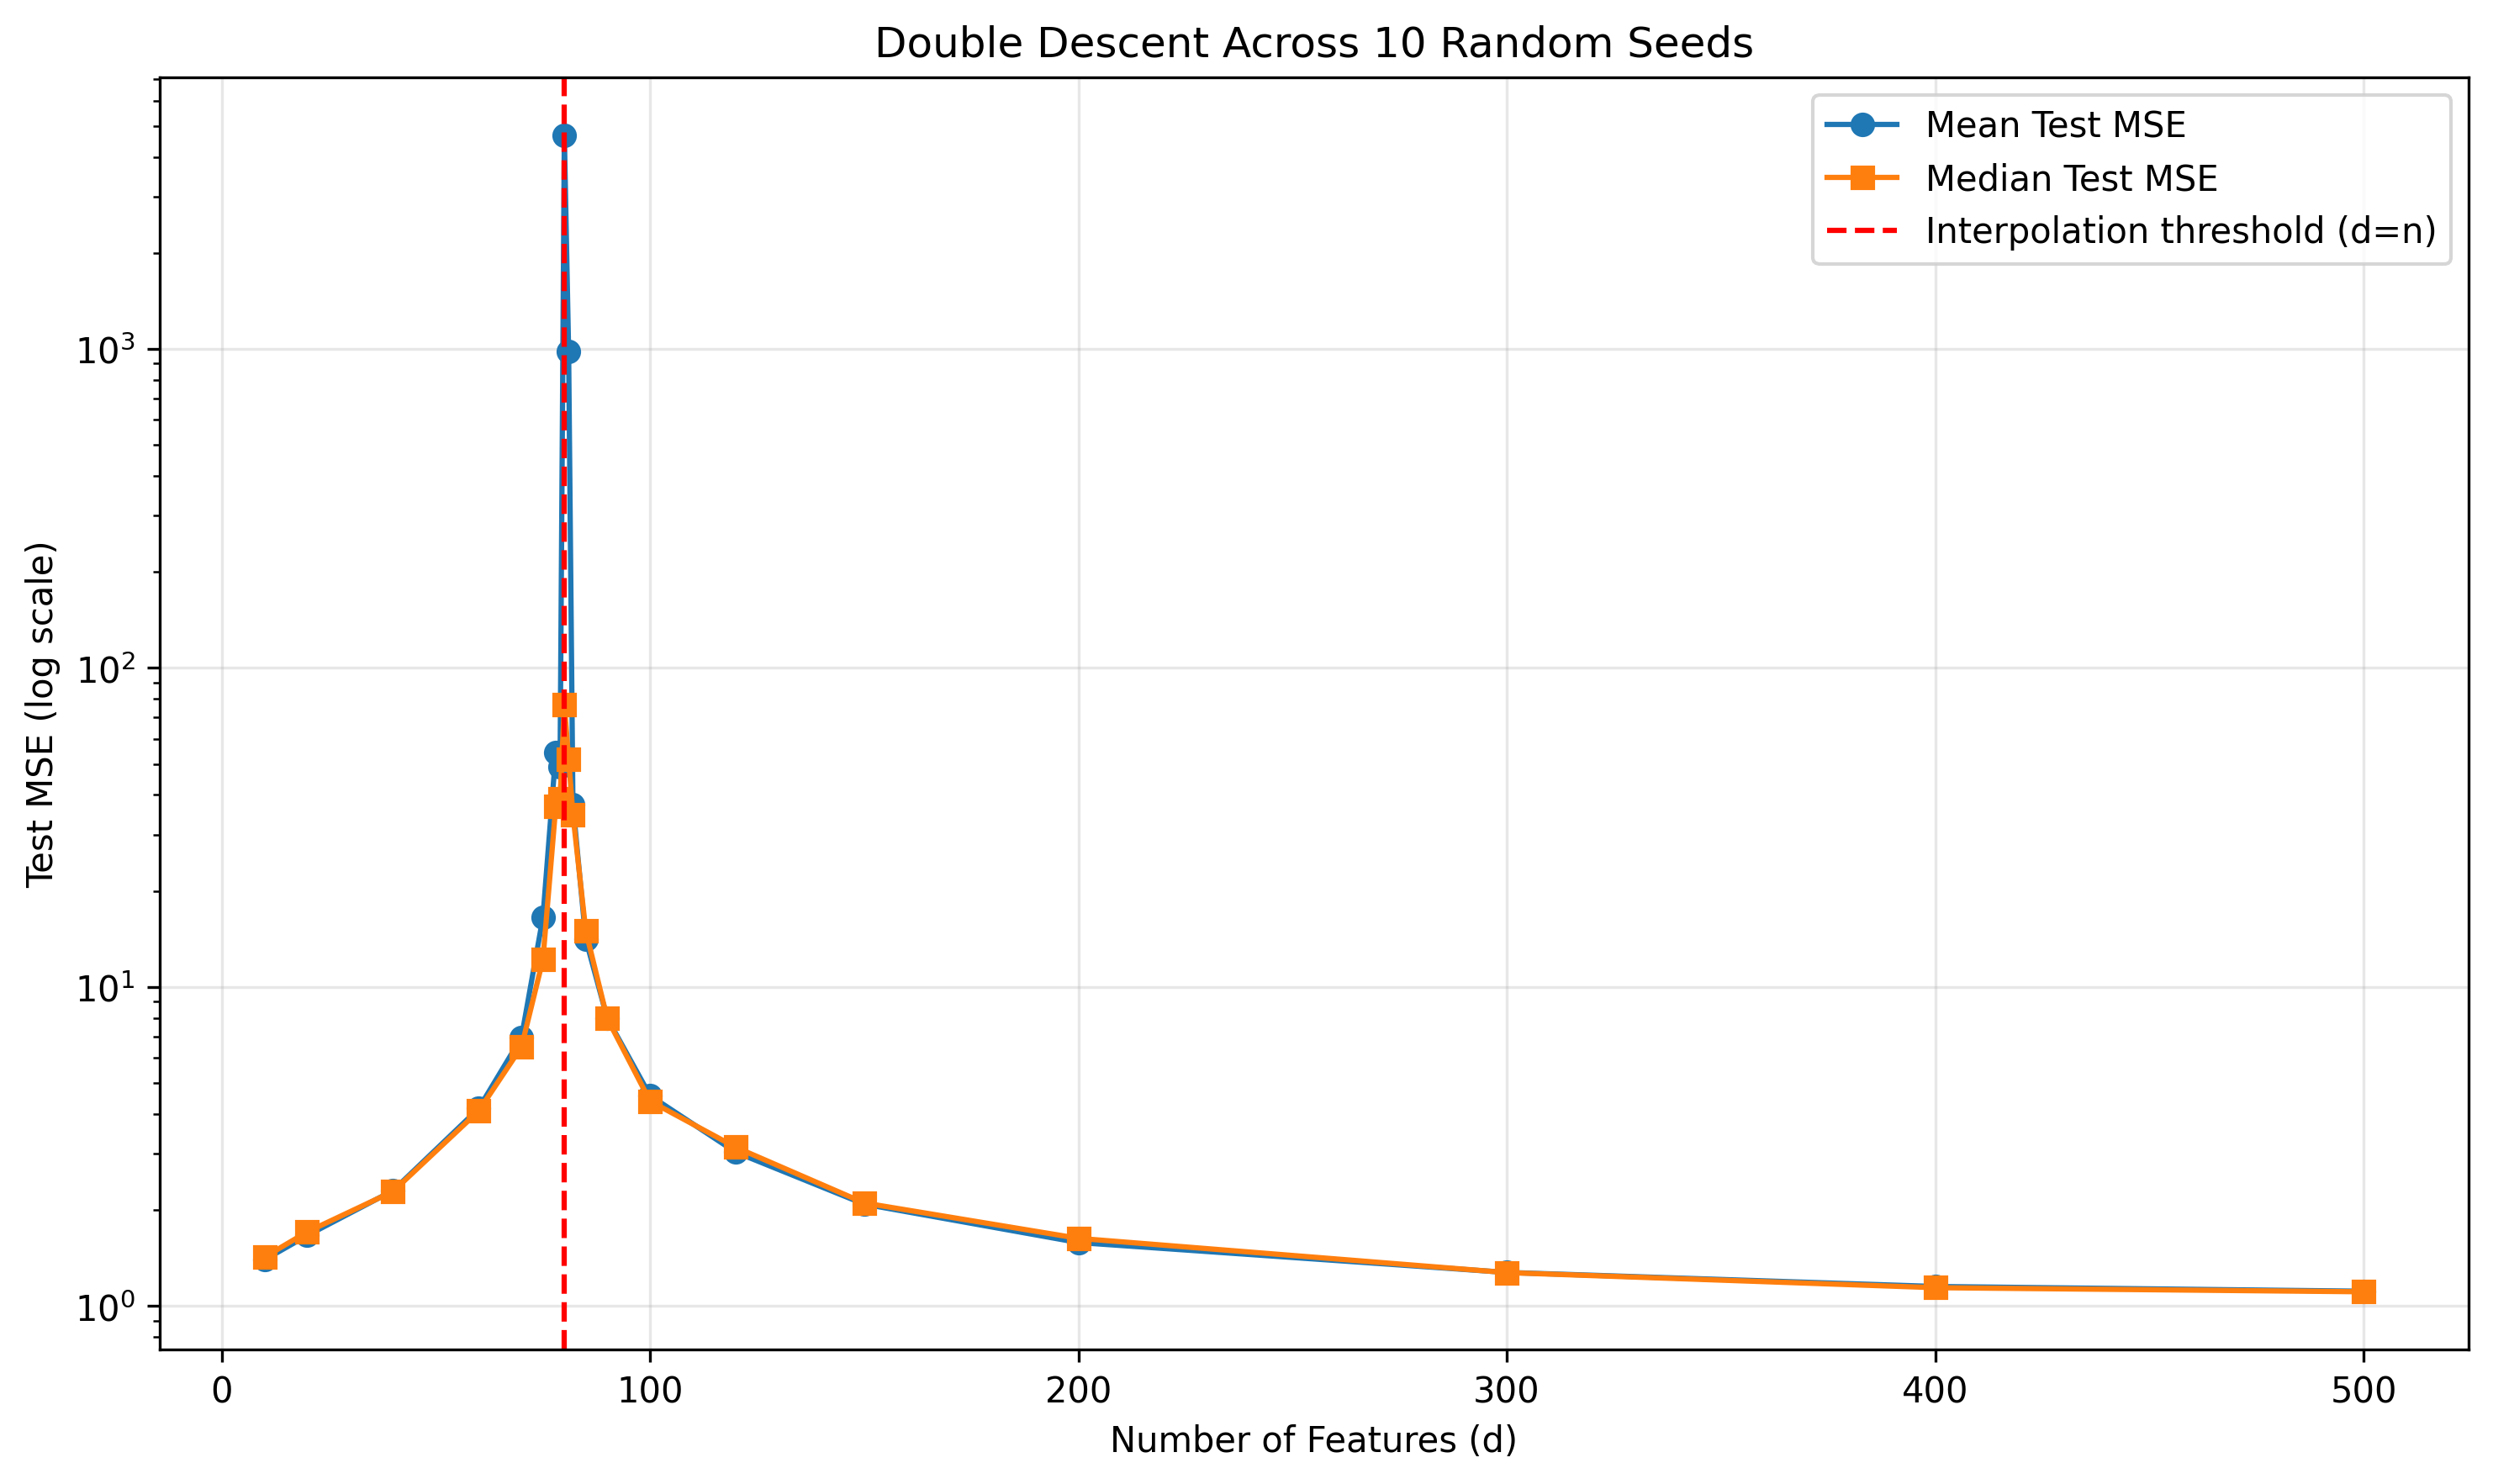
\includegraphics[width=0.85\textwidth]
    {synthetic_repeated_experiments.png}
    \caption{Double descent across 10 random seeds.
    The plot summarizes the mean and median test
    errors at each feature dimension.}
    \label{fig:synthetic_seeds}
\end{figure}

The interpolation peak is visible in both
the mean and median results.
At $d=80$, the mean test MSE is approximately
$4{,}680.83$, while the median is approximately
$76.70$.
The large difference indicates that some
random runs produce exceptionally high errors,
which strongly influence the mean.
At $d=500$, the mean and median test errors
are approximately $1.11$.
This suggests that the extreme instability is
concentrated near the interpolation threshold.

\subsection{Effect of Label Noise}
We also examined label noise with standard
deviations of $0.1$, $0.5$, and $1.0$.

\begin{figure}[htbp]
    \centering
    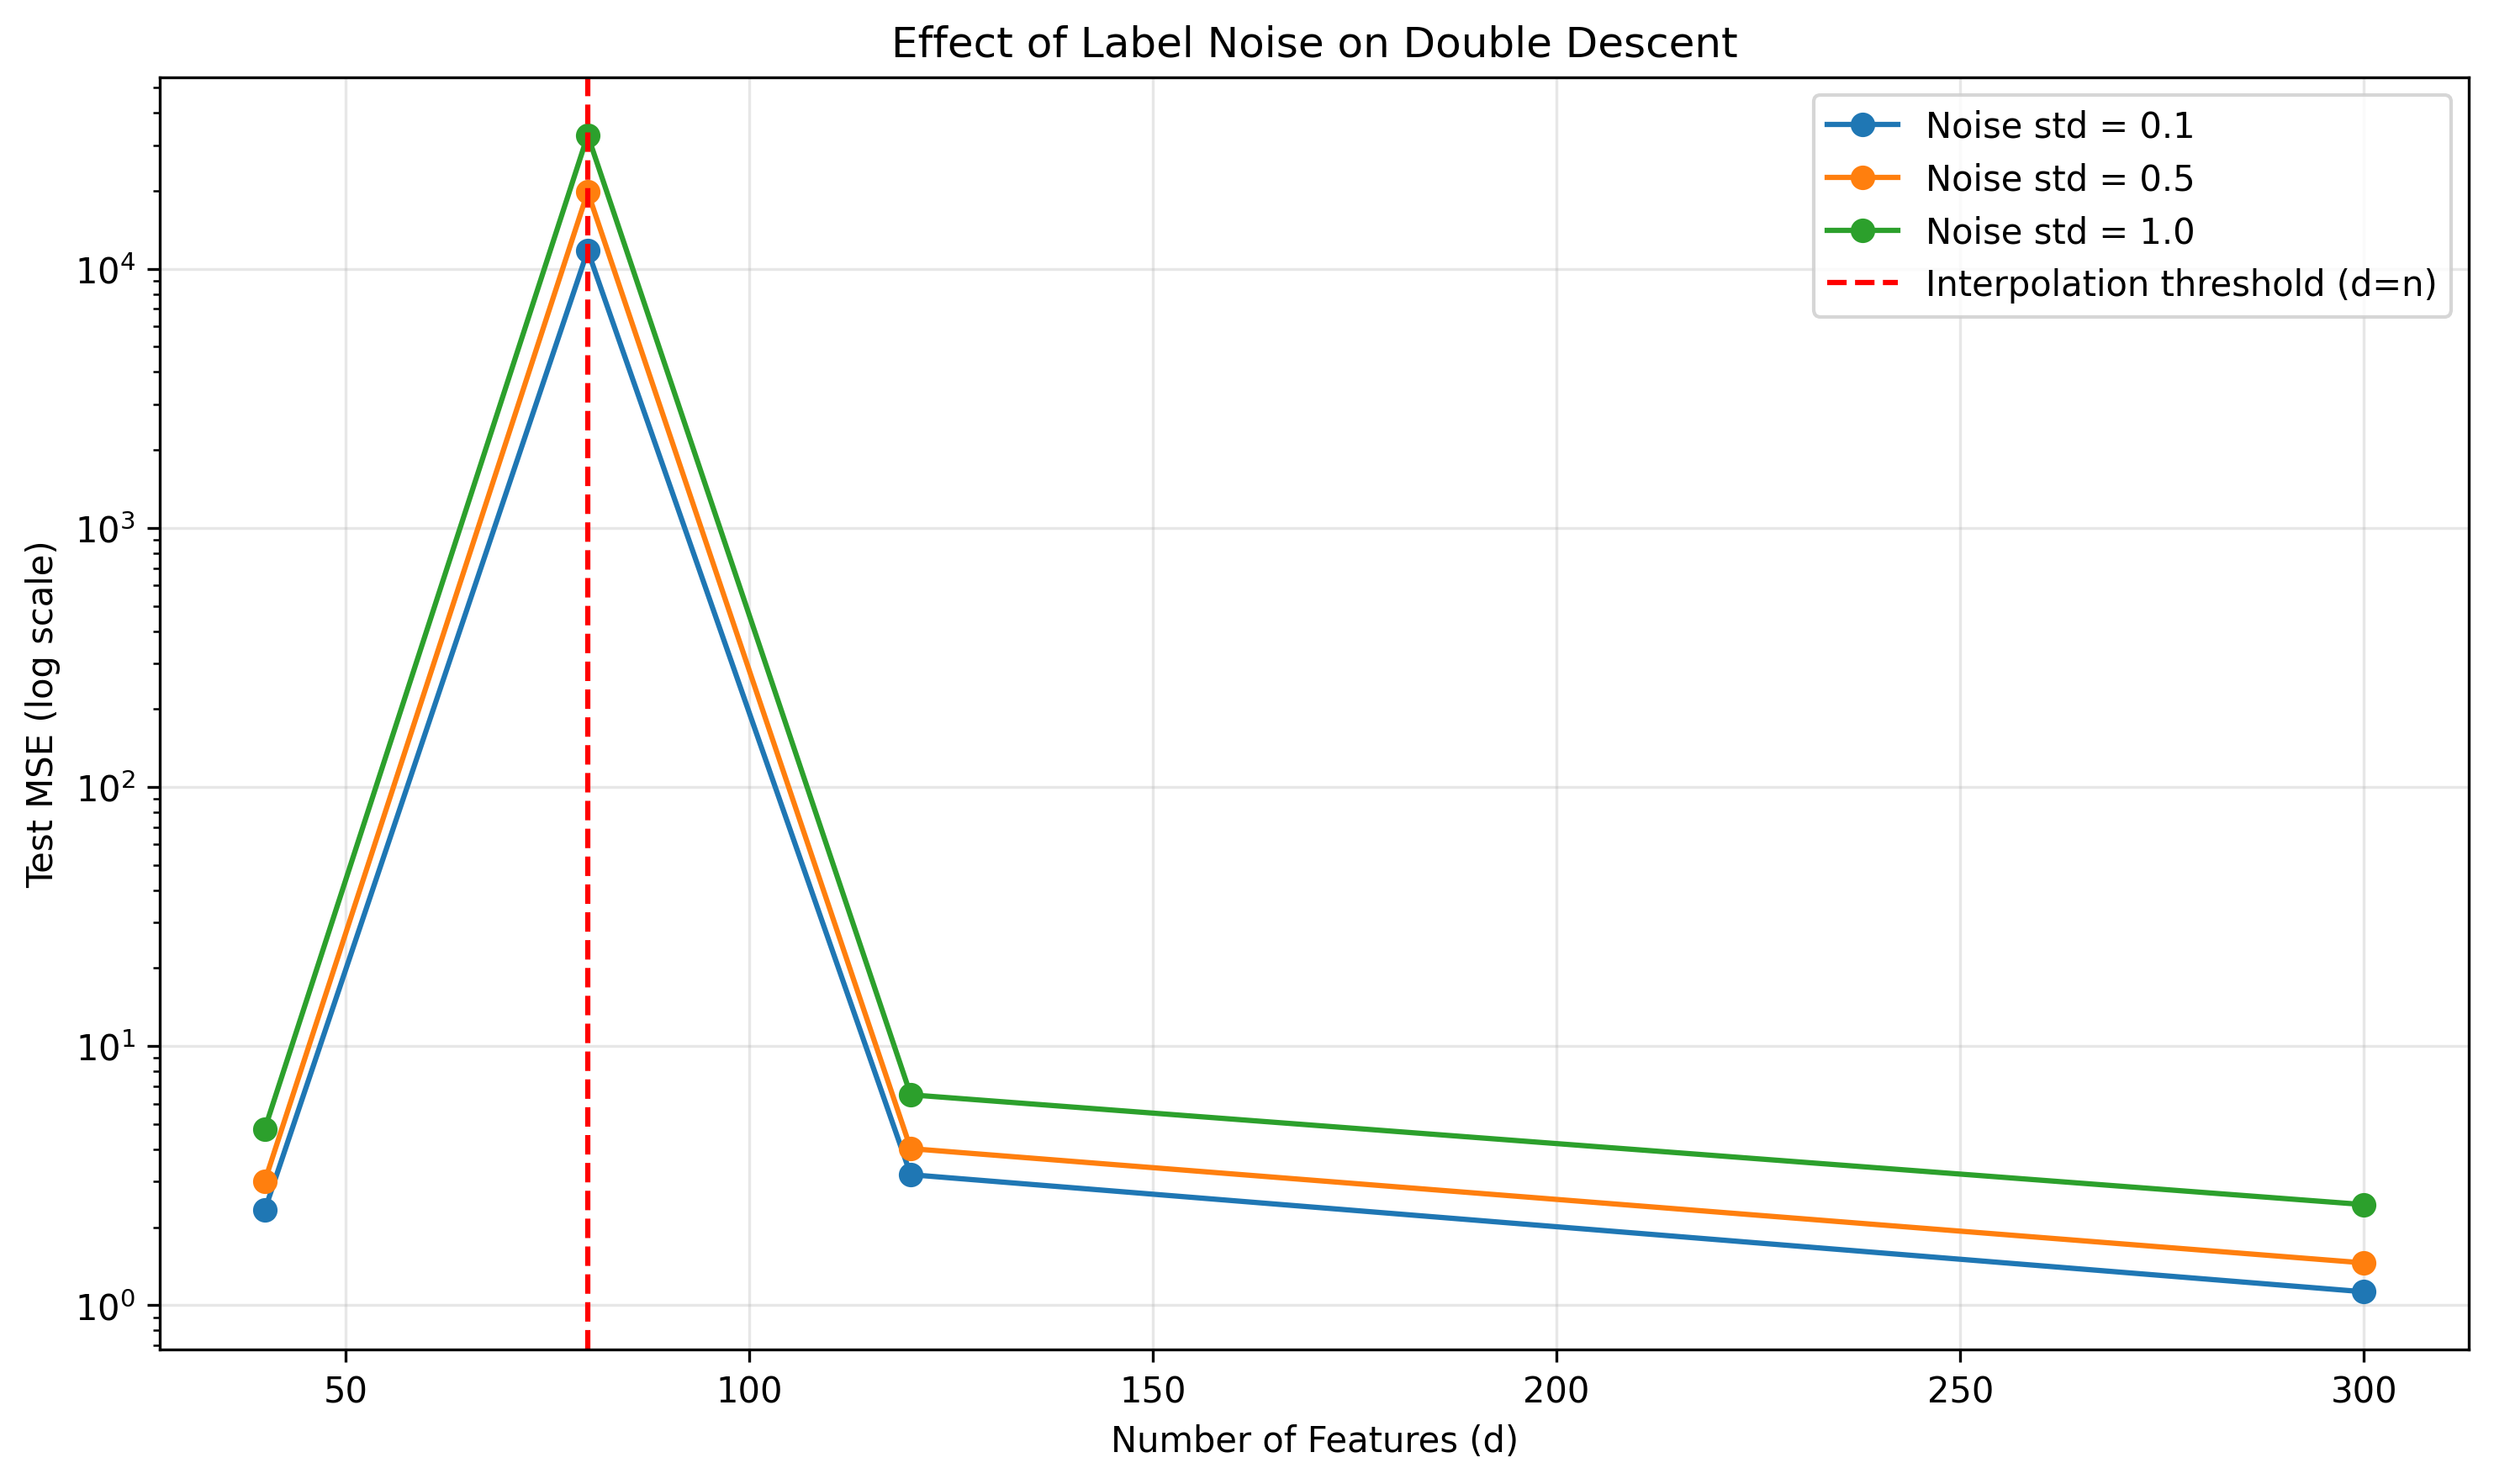
\includegraphics[width=0.85\textwidth]
    {synthetic_noise_effect.png}
    \caption{Effect of increasing label noise
    on least squares test error. The experiment
    uses a fixed random seed and compares
    four feature dimensions.}
    \label{fig:synthetic_noise}
\end{figure}

At $d=80$, test MSE increases from approximately
$11{,}763.17$ with low noise to $32{,}779.51$
with high noise.
Increasing label noise raises test error at
all four investigated feature dimensions.
Nevertheless, the decrease in test error
after the interpolation threshold is visible
at all three noise levels.
Since this experiment uses only one random seed,
the results should be interpreted as an
illustration rather than a statistical estimate
of the general effect of noise.

\subsection{Sparse and Dense Signal Comparison}
The dense-signal experiments exhibit a clear
second descent after the interpolation peak.
In contrast, the sparse-signal experiment
shows a large interpolation peak but does not
exhibit the same sustained improvement at
large feature dimensions.
This distinction indicates that the observed
generalization behavior depends not only on
model complexity but also on the structure of
the underlying signal and the features included
in the model.

\section{California Housing Experimental Results}
We investigated whether double descent also appears
when using a real-world regression dataset.
The California Housing dataset contains eight original
input features. We used Random Fourier Features (RFF)
to construct higher-dimensional representations.
The training sample size was fixed at $n=100$, while
the number of transformed features increased from
$d=10$ to $d=300$.

\subsection{Double Descent in Least Squares}
Figure~\ref{fig:california_dd} presents the training
and test errors obtained using least squares.

\begin{figure}[htbp]
    \centering
    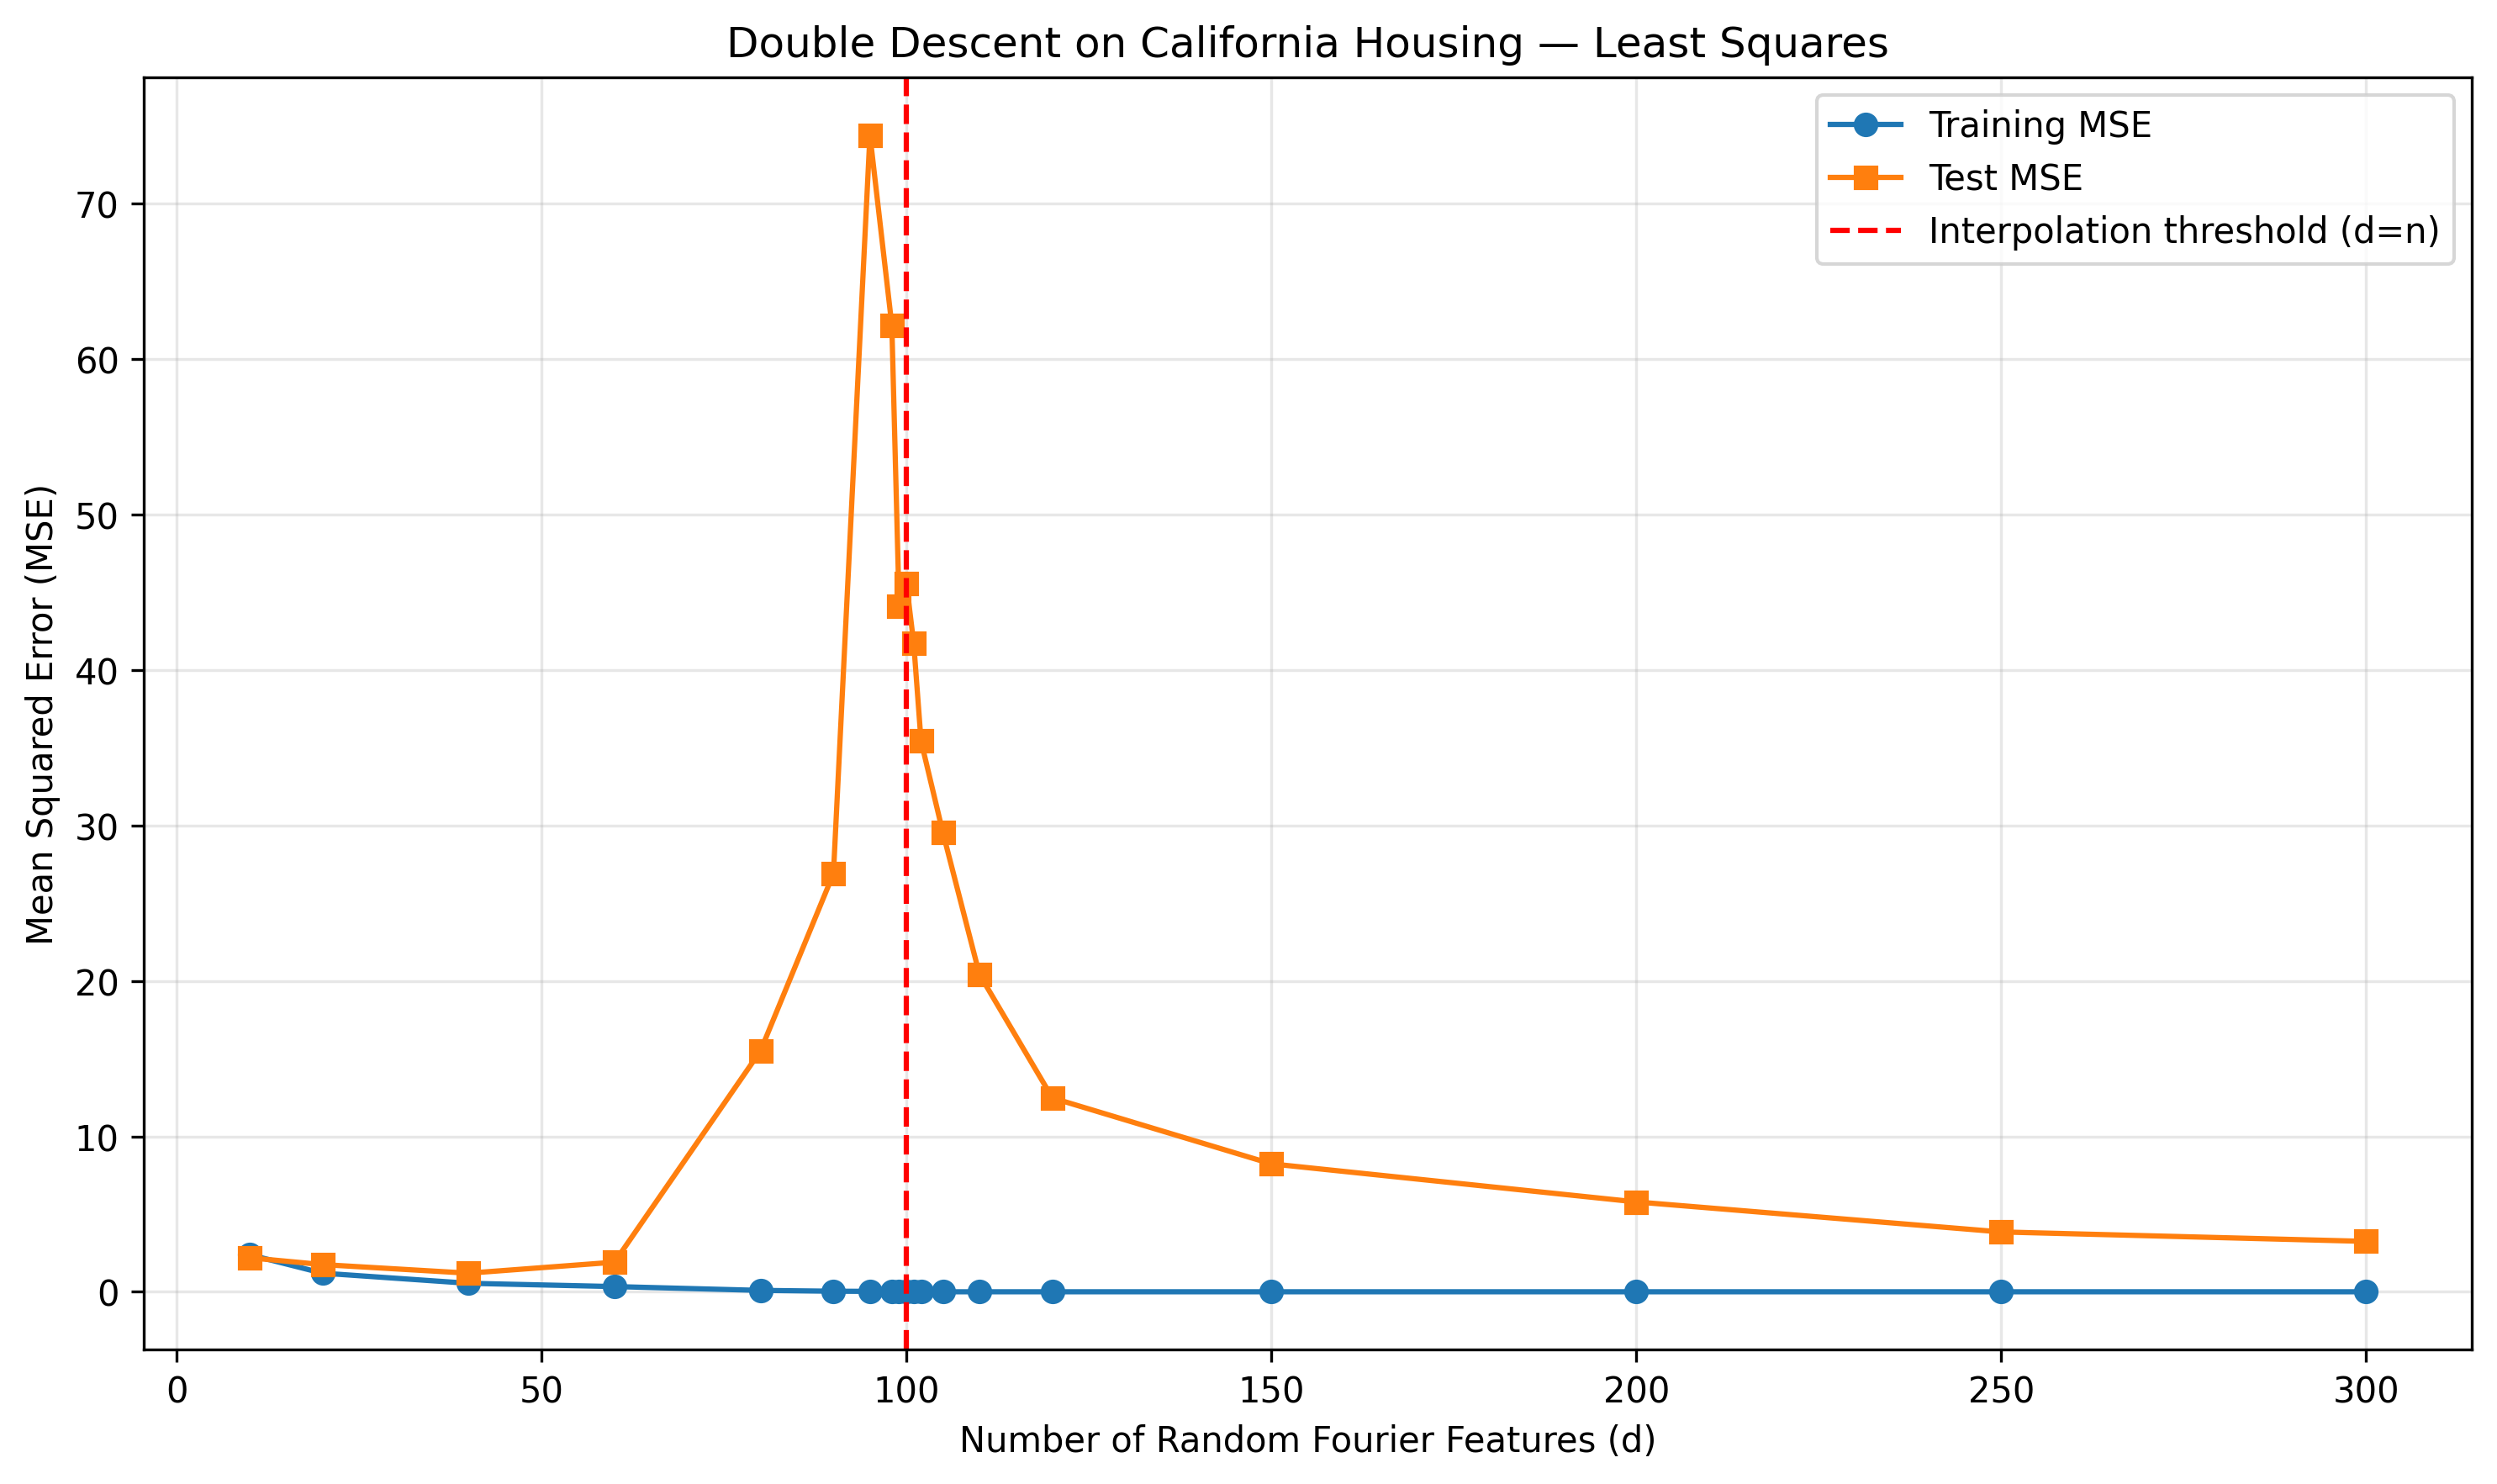
\includegraphics[width=0.82\textwidth]
    {california_double_descent.png}
    \caption{Training and test MSE for least squares
    regression on California Housing using Random
    Fourier Features. The interpolation threshold
    is near $d=100$.}
    \label{fig:california_dd}
\end{figure}

The test error increases sharply near the
interpolation threshold.
The largest observed test MSE occurs at $d=95$,
where the error reaches approximately $74.40$.
At $d=100$, the test MSE is approximately $45.56$.
After the interpolation region, the test error
decreases substantially, reaching approximately
$3.24$ at $d=300$.
However, this final error remains higher than
the test MSE of approximately $1.20$ observed
at $d=40$.
Therefore, the experiment demonstrates a
pronounced interpolation peak and a subsequent
decrease in error, but not an improvement
beyond the best underparameterized model.

\subsection{Least Squares versus Ridge Regression}
We compared least squares with Ridge Regression
using a fixed regularization parameter $\alpha=1$.

\begin{figure}[htbp]
    \centering
    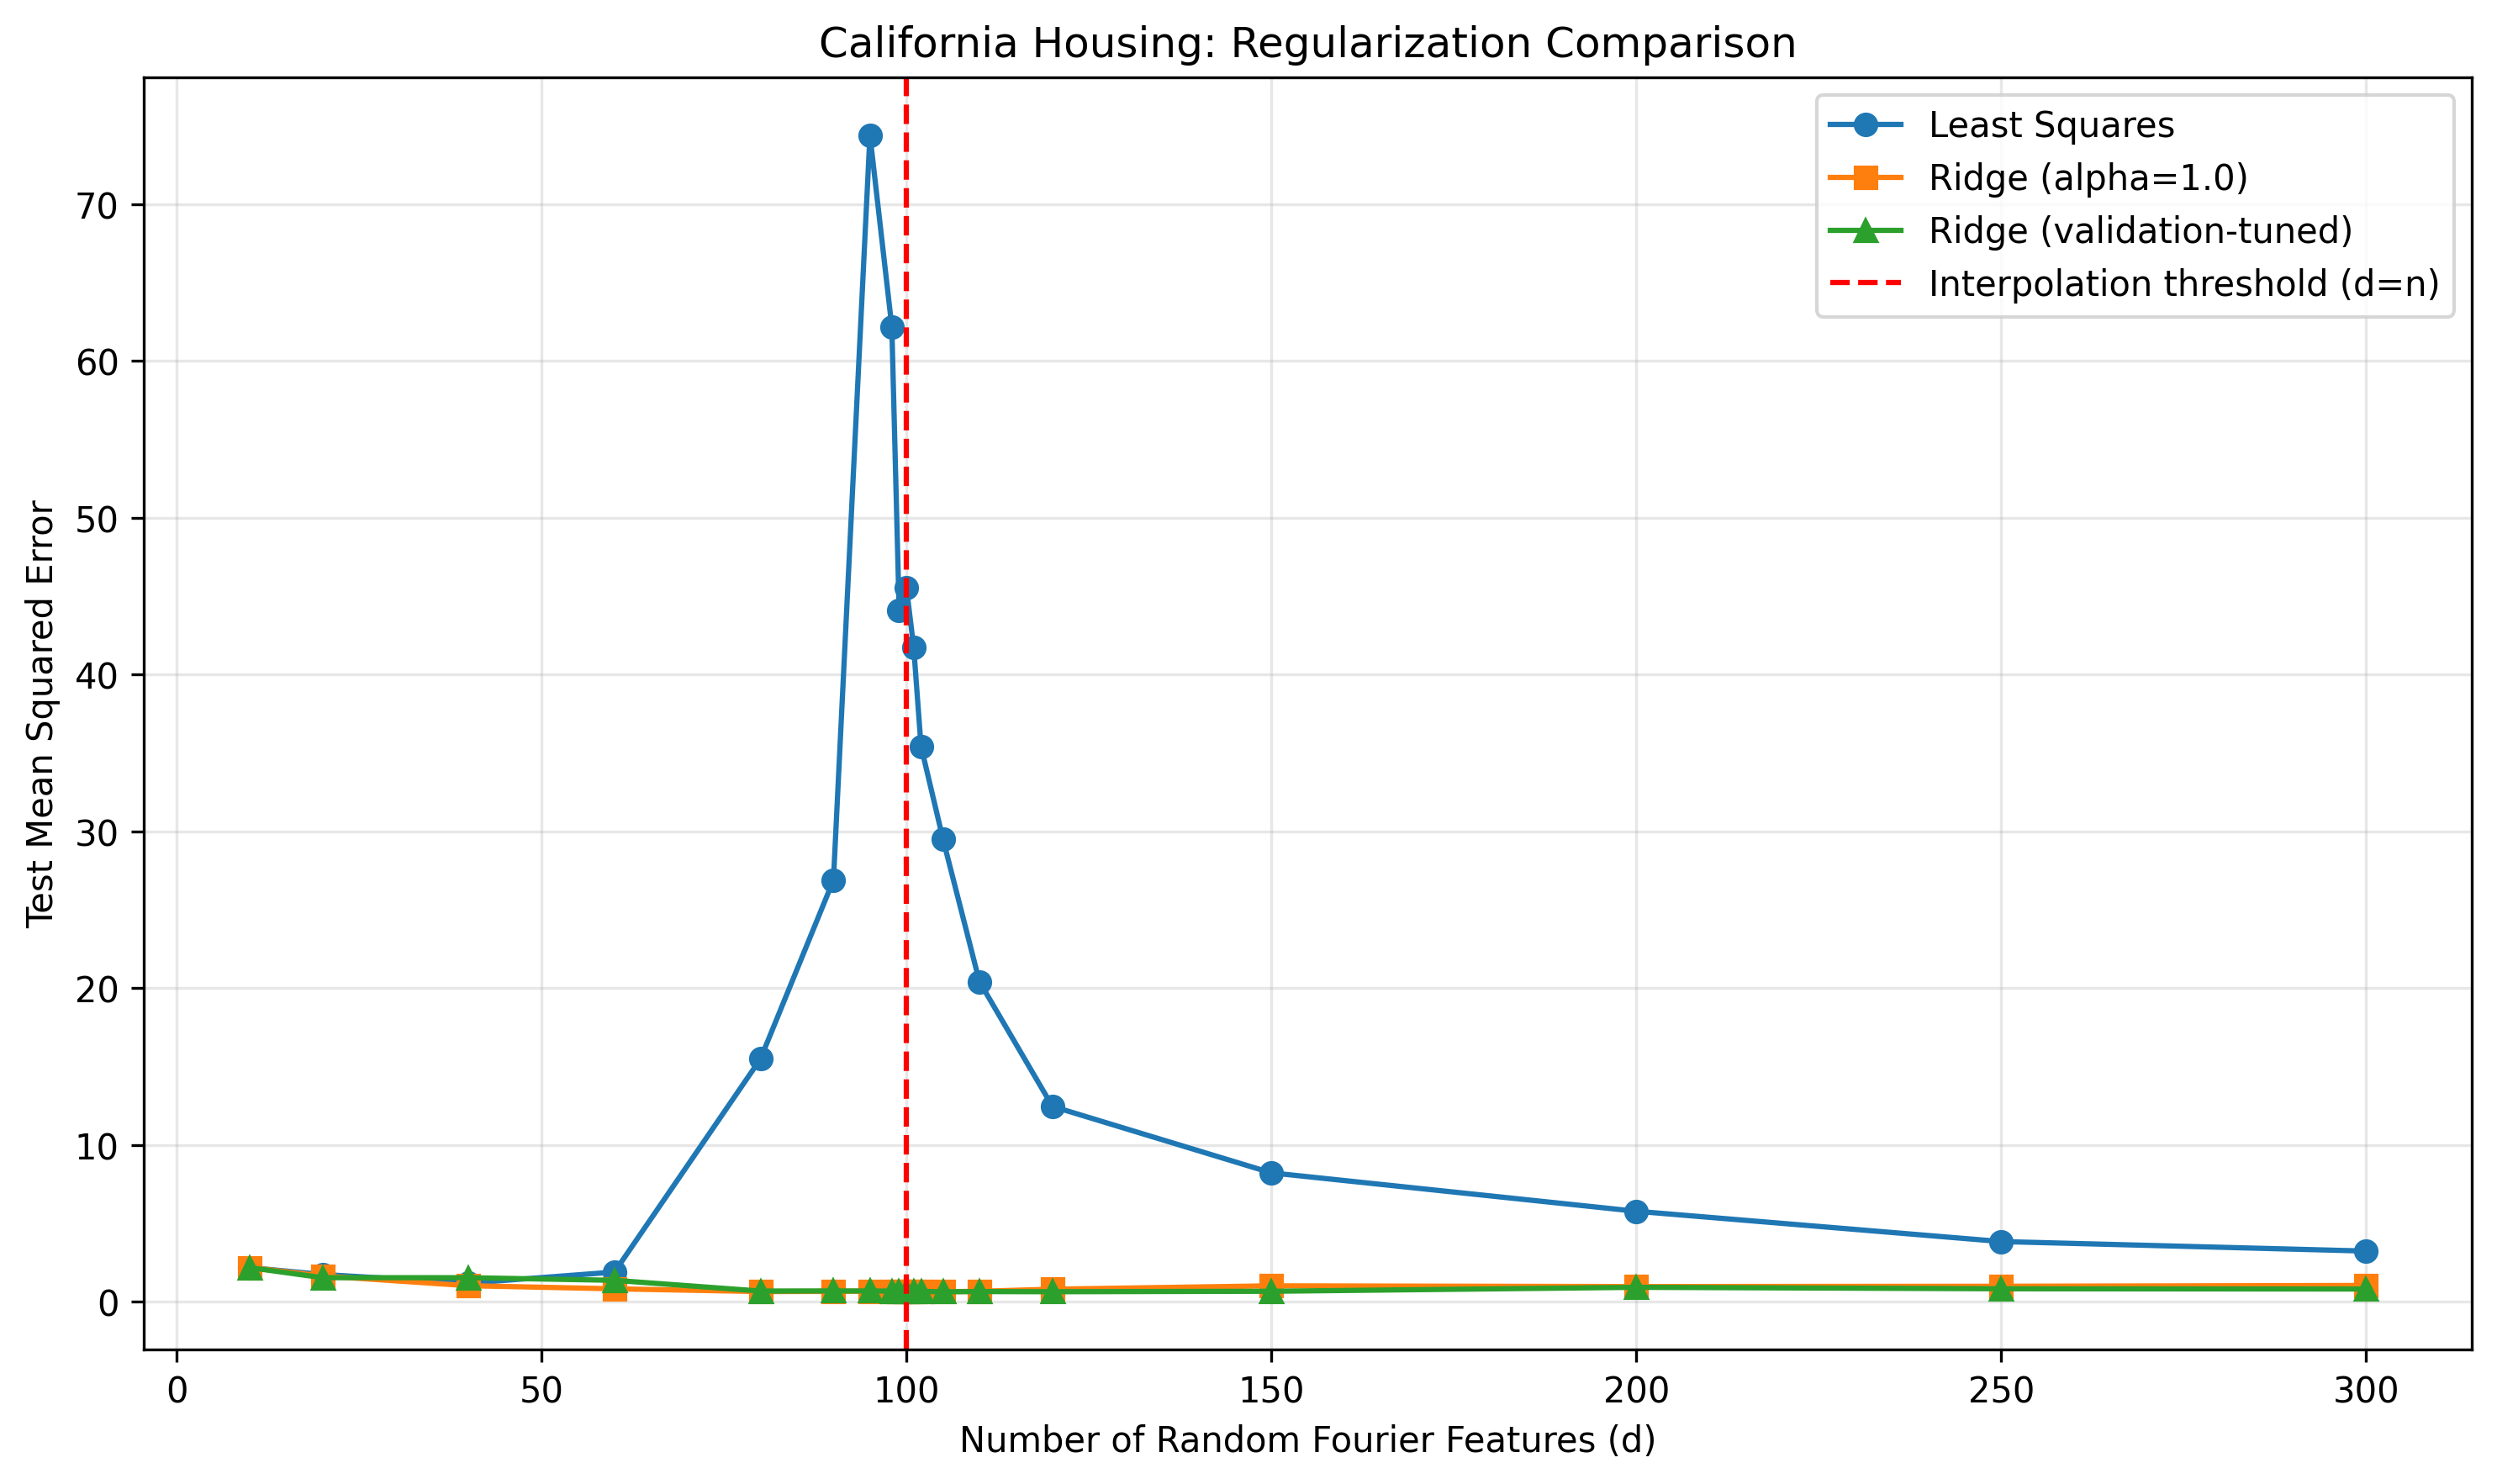
\includegraphics[width=0.82\textwidth]
    {california_regularization_comparison.png}
    \caption{Least squares and Ridge Regression
    test MSE across different numbers of Random
    Fourier Features. Ridge uses $\alpha=1$.}
    \label{fig:california_ridge}
\end{figure}

Ridge Regression produces substantially lower
test error around the interpolation threshold.
For example, at $d=100$, the least-squares
test MSE is approximately $45.56$, whereas
Ridge Regression achieves approximately $0.67$.
The results indicate that regularization
can substantially reduce the instability
associated with interpolation.

\subsection{Validation-Based Ridge Tuning}
We also selected the Ridge regularization
parameter separately for each feature dimension.
The candidate values were
$\{0.01,0.1,1,10,100\}$.
The best value was selected using validation
MSE, and the selected model was evaluated
on the test set.

\begin{figure}[htbp]
    \centering
    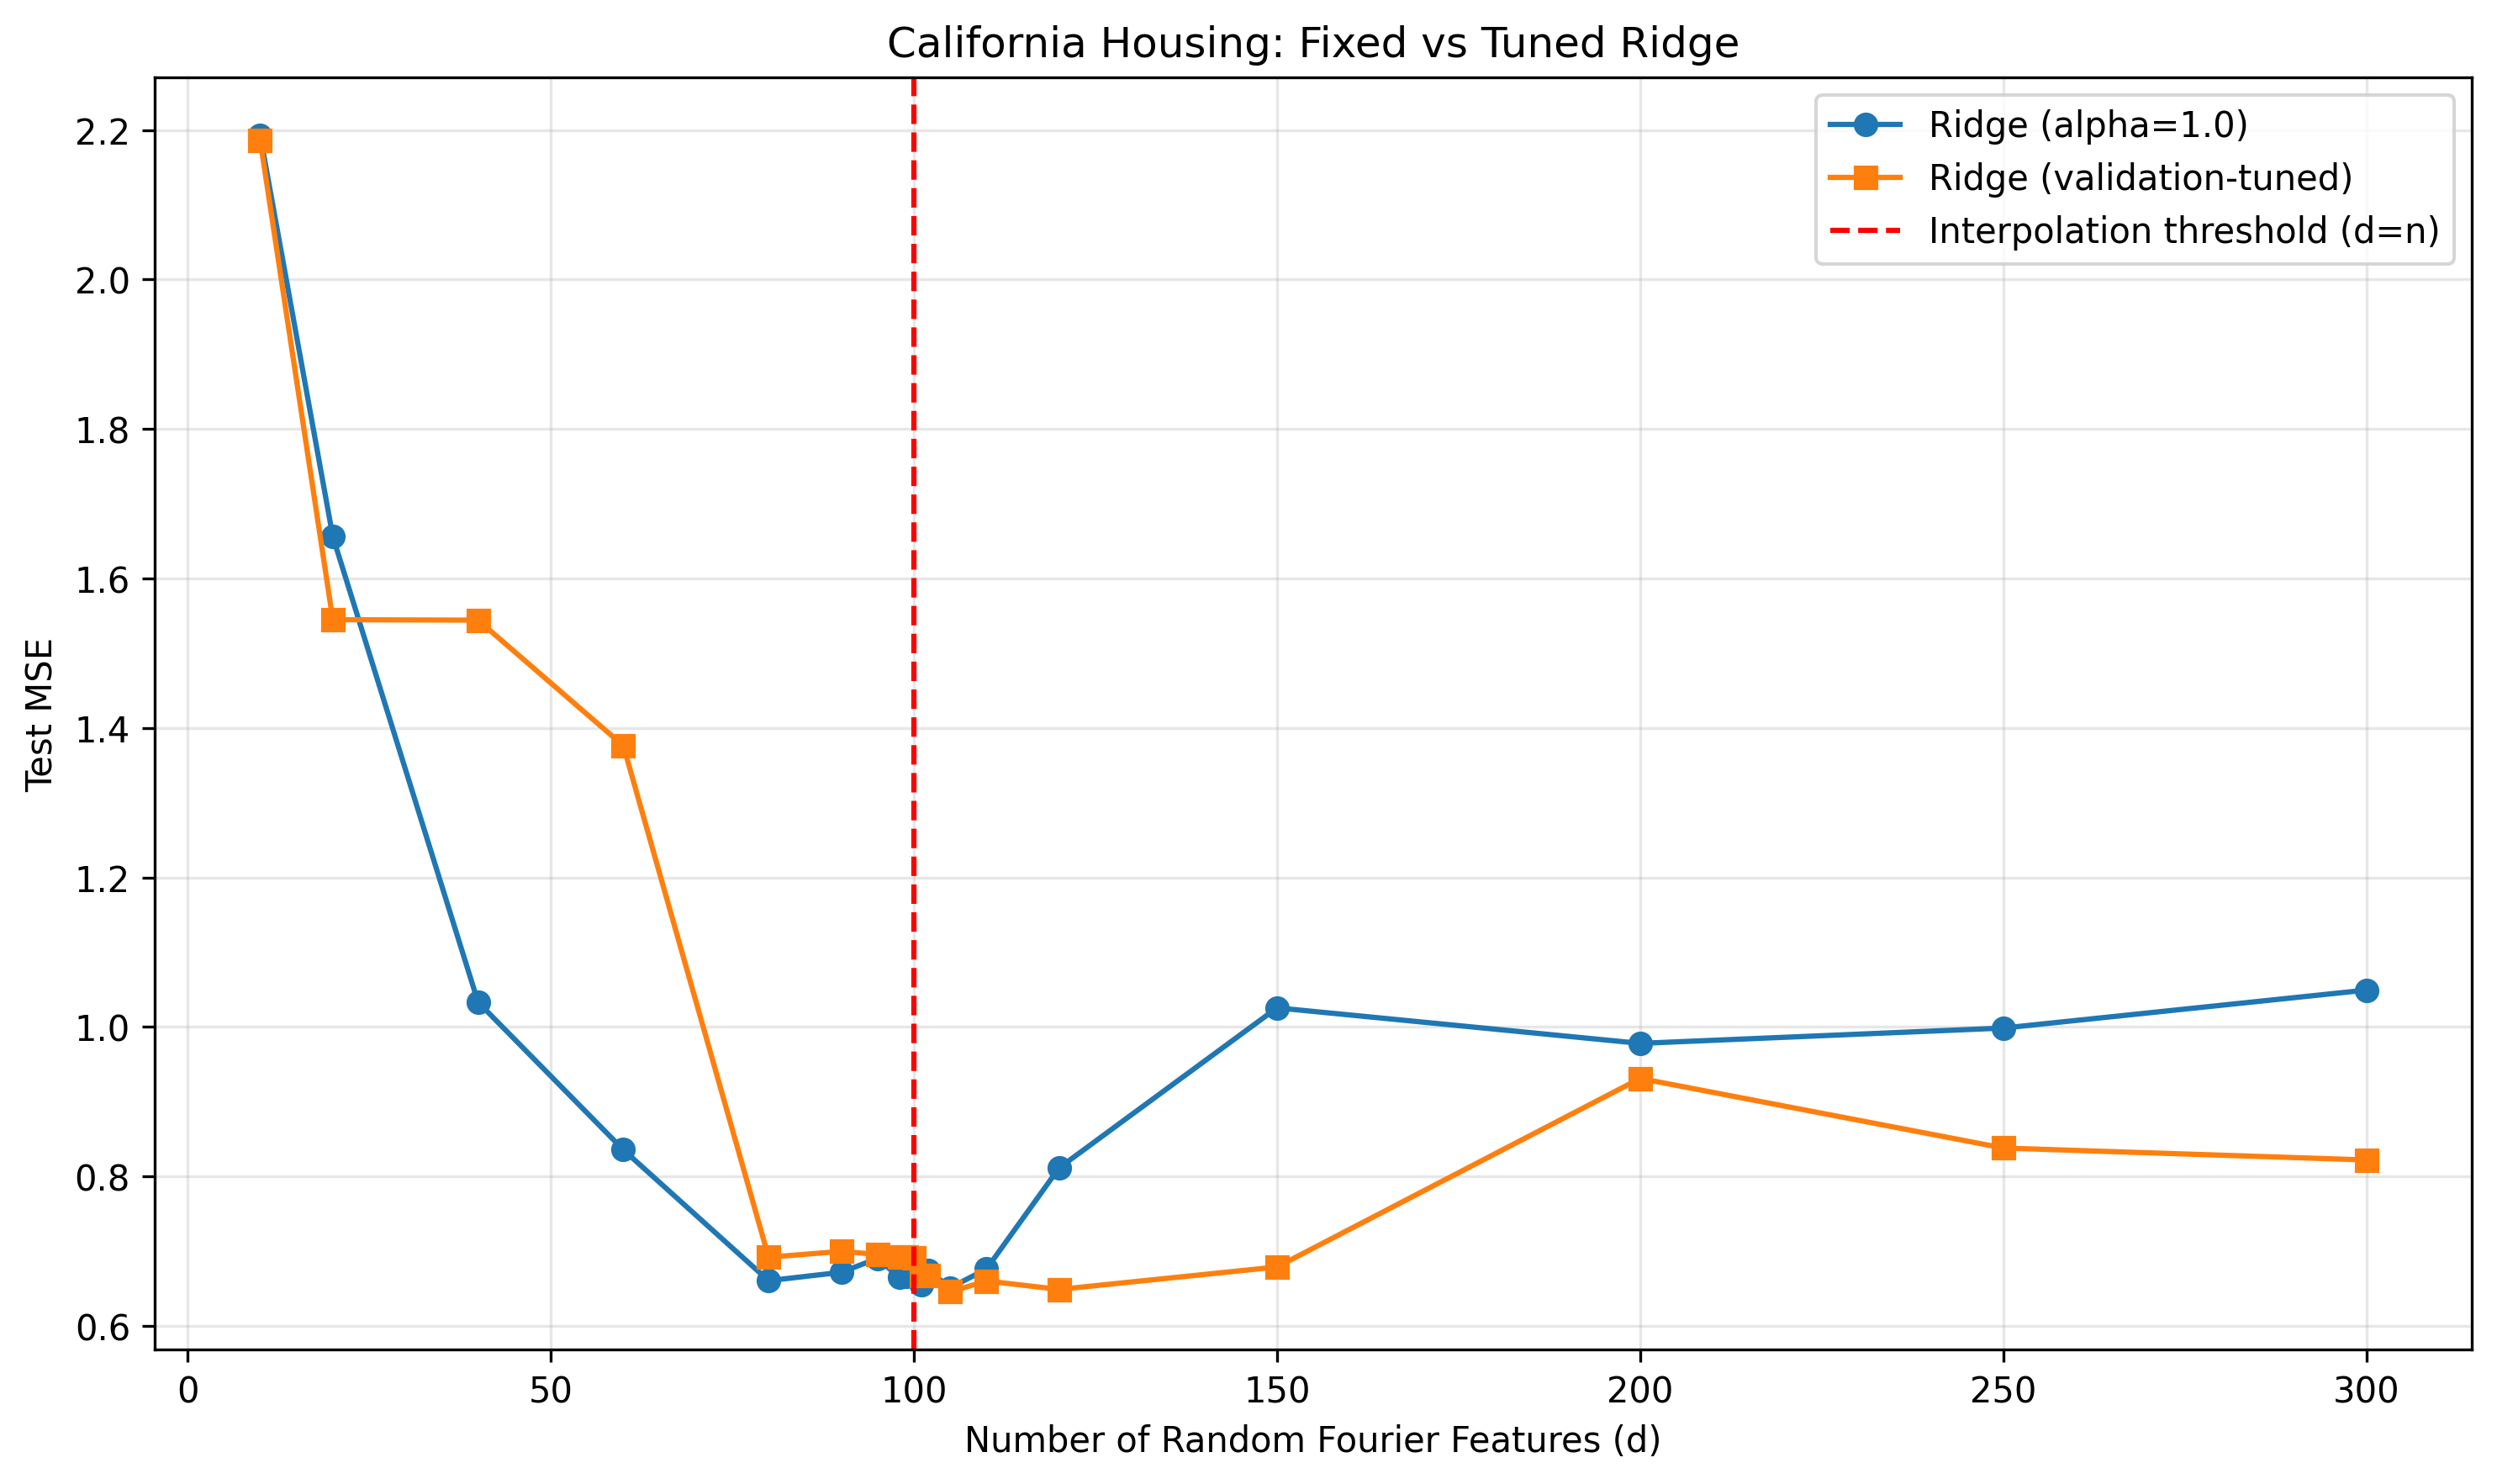
\includegraphics[width=0.82\textwidth]
    {california_ridge_tuning.png}
    \caption{Comparison of fixed Ridge regularization
    ($\alpha=1$) and Ridge regularization selected
    using validation data.}
    \label{fig:california_tuning}
\end{figure}

At $d=100$, validation-based tuning selected
$\alpha=10$.
The corresponding test MSE was approximately
$0.69$, compared with approximately $0.67$
for fixed $\alpha=1$.
Although the validation-selected parameter
did not achieve a lower test error at this
particular dimension, it was selected without
using test-set information.
At $d=300$, the validation-selected model
achieved a test MSE of approximately $0.82$.
These results demonstrate that validation-based
selection provides a systematic method for
choosing regularization strength, although
it does not guarantee the lowest test error
for every particular dataset split.

\subsection{Comparison with Synthetic Experiments}
Figure~\ref{fig:final_comparison} compares
the least-squares test-error curves from the
synthetic dense-signal and California Housing
experiments.

\begin{figure}[htbp]
    \centering
    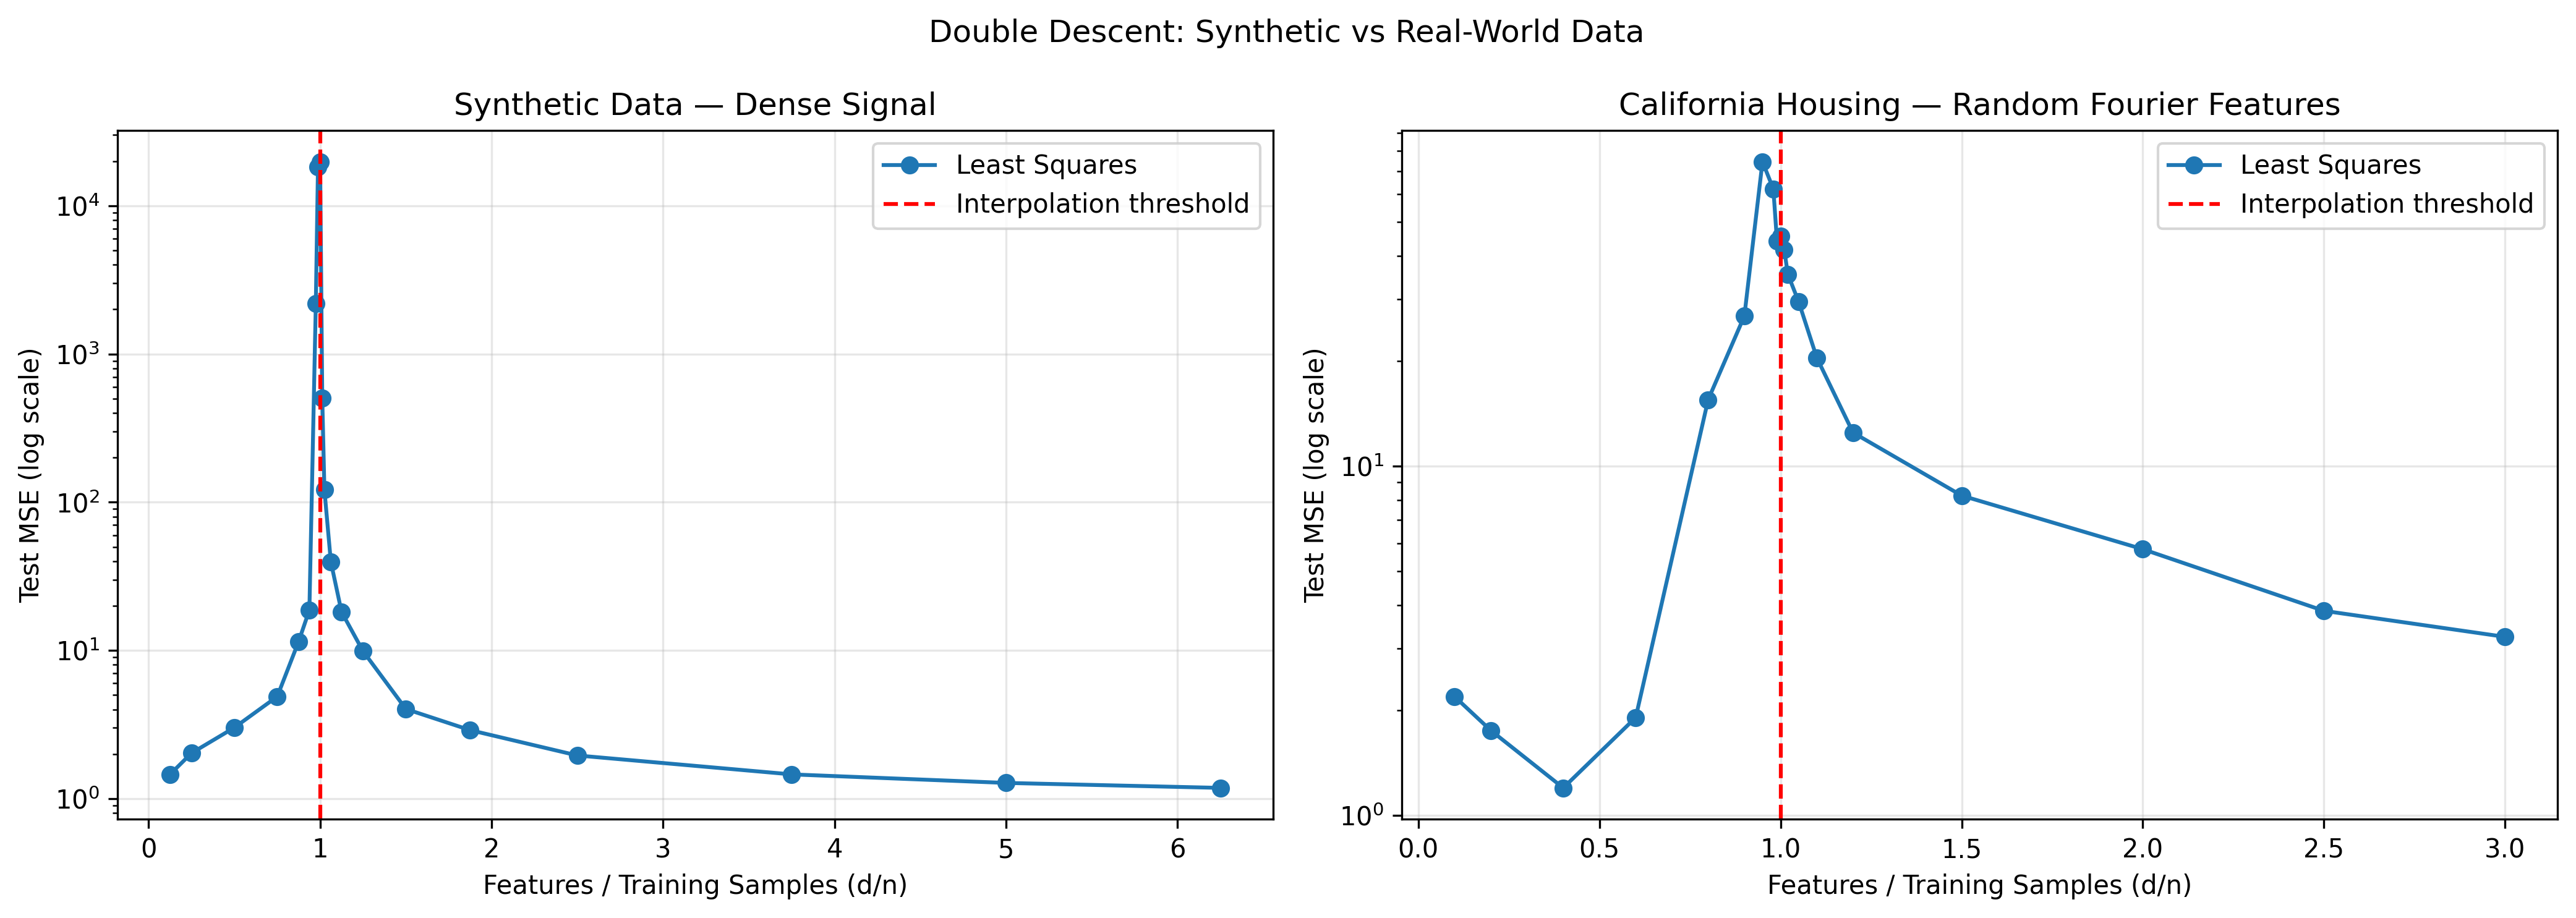
\includegraphics[width=\textwidth]
    {final_dataset_comparison.png}
    \caption{Comparison of double descent in
    synthetic and real-world regression.
    The horizontal axis shows the ratio $d/n$,
    and each panel has its own logarithmic
    test-error scale.}
    \label{fig:final_comparison}
\end{figure}

Both experiments display a substantial increase
in test error near the interpolation threshold,
followed by a decrease in the overparameterized
regime.
However, the synthetic dense-signal experiment
shows a much stronger second descent relative
to its earlier test-error values.
This difference illustrates how the behavior
of overparameterized regression depends on
the underlying data and feature representation.

\section{Discussion}
The experiments demonstrate that the relationship
between model complexity and generalization error
is not always described by the classical
bias-variance trade-off.
In both the synthetic dense-signal experiment
and the California Housing experiment,
least squares exhibits a pronounced increase
in test error near the interpolation threshold,
followed by a decrease in the overparameterized
regime.

\subsection{Understanding the Interpolation Peak}
The interpolation peak appears when the
number of features approaches the number
of training observations.
Near this threshold, the design matrix may
become poorly conditioned, making the
least-squares solution highly sensitive
to noise and small changes in the data.
The dense-signal synthetic experiment
demonstrates this behavior particularly
clearly, with a test MSE exceeding 19,000
at $d=80$.
The repeated-seed experiment also shows
that some random datasets produce much
larger errors than others near interpolation.

\subsection{The Role of Regularization}
Ridge regression substantially reduces
the interpolation peak in both datasets.
By penalizing large coefficient values,
ridge regularization reduces the sensitivity
of the estimated parameters to poorly
conditioned feature matrices.
Our experiments therefore support the
importance of regularization when fitting
models near the interpolation threshold.
However, increasing regularization does
not always improve test error. The optimal
choice depends on the data and should be
determined through an appropriate
validation procedure.

\subsection{Signal Structure and Generalization}
The synthetic experiments demonstrate that
the structure of the target signal affects
the shape of the test-error curve.
In the dense-signal experiment, test error
decreases considerably in the
overparameterized regime.
The sparse-signal experiment does not
exhibit the same sustained second descent.
This difference suggests that increasing
the number of features is not automatically
beneficial. The relationship between the
features and the true signal is also
important.

\section{Limitations}
Although the experiments illustrate
important aspects of double descent,
several limitations should be considered.
\begin{enumerate}
    \item \textbf{Limited training sample sizes.}
    The synthetic experiments use 80
    training observations, while the
    California Housing experiments use 100.
    Larger samples could produce
    different results.
    \item \textbf{Random variation.}
    The main experimental curves use
    fixed random seeds. Although one
    synthetic experiment was repeated
    across 10 seeds, not all experiments
    include repeated trials.
    \item \textbf{Noise analysis.}
    The noise experiment uses one
    random seed and four feature
    dimensions. It illustrates a
    pattern but does not establish
    its statistical reliability.
    \item \textbf{Validation set size.}
    Ridge hyperparameters for California
    Housing were selected using only
    30 validation observations.
    This may make parameter selection
    sensitive to the particular split.
    \item \textbf{Feature representation.}
    The California Housing experiment
    uses randomly generated Fourier
    features. Different random
    projections or kernel settings
    may change the error curves.
    \item \textbf{Finite feature range.}
    We investigate only selected
    feature dimensions. The results
    do not establish how test error
    would behave at arbitrarily
    large model sizes.
\end{enumerate}


\section{Conclusion}
This project investigated the double
descent phenomenon in linear regression
using synthetic data and the California
Housing dataset.
The main experiments show that least
squares test error can increase sharply
near the interpolation threshold and
decrease again as the number of
features grows beyond the number
of training observations.
Ridge regularization substantially
reduces the interpolation peak,
demonstrating the value of controlling
model complexity through
regularization.
The experiments also show that label
noise, random variation, and the
underlying signal structure influence
generalization performance.
Overall, the findings illustrate
that overparameterization does not
necessarily lead to monotonically
worse generalization, and that
the relationship between model
complexity and prediction accuracy
depends on the learning algorithm,
regularization, and data.
Future work could investigate
larger datasets, additional random
seeds, and different feature
representations.

\section*{Academic Integrity Declaration}
I declare that this report and the accompanying code represent my own work.
Any external sources used have been acknowledged. I have not presented
another person's work as my own.\par

\begin{thebibliography}{9}
    \bibitem{belkin2019}
    Belkin, M., Hsu, D., Ma, S., and Mandal, S. (2019).
    Reconciling modern machine-learning practice
    and the classical bias-variance trade-off.
    \textit{Proceedings of the National Academy of Sciences},
    116(32), 15849--15854.
    \end{thebibliography}
\end{document}
